\documentclass[review,authoryear]{elsarticle}

\usepackage[list-units=single]{siunitx}
\usepackage{cleveref}
\usepackage{amsmath}
\usepackage{graphicx}

\usepackage[modulo]{lineno}

\makeatletter
\g@addto@macro\@floatboxreset\centering
\makeatother

\journal{Ocean Modelling}
% Harvard-style author-year bibliography
\bibliographystyle{model2-names}

\begin{document}

\begin{frontmatter}
\title{The orientation of spurious mixing}
\author[anu]{Angus~H.~Gibson}
\ead{angus.gibson@anu.edu.au}
\author[anu]{Andrew~McC.~Hogg}
\author[unsw]{Andrew~E.~Kiss}
\address[anu]{Research School of Earth Sciences, Australian National University, Canberra, Australian Capital Territory, Australia}
\address[unsw]{School of Physical, Environmental and Mathematical Sciences, University of New South Wales at the Australian Defence Force Academy, Canberra, Australian Capital Territory, Australia}

\begin{abstract}
  Some stuff about spurious mixing, we found out about its orientation
\end{abstract}

\end{frontmatter}

% start numbering lines from here
\linenumbers

\section{Introduction}

One of the myriad uses of ocean models is in developing ocean heat uptake estimates and overturning circulation predictions \citep{armour16}. Additionally, the overturning circulation itself affects the wider climate, which manifests when ocean models are used as a component of coupled climate simulations. The problems of ocean heat uptake and overturning circulation are both strongly defined by the density structure of the ocean, which is modified by mixing. For example, mixing at depth controls the abyssal overturning cell that constitutes part of the meridional overturning circulation \citep{mashayek15}. Additionally, the time scale of adjustment of overturning circulation toward equilibrium depends primarily on mixing near the surface \citep{vreugdenhil15}. As a result, models may be unable to accurately constrain the abyssal overturning if the magnitude of spurious diapycnal mixing cannot be completely controlled.

% TODO define "spurious diapycnal mixing" here?

Numerical ocean models are governed by approximations of the incompressible Navier-Stokes equations for momentum, also known as the primitive equations \citep{griffies04}. In these models, the vertical balance is hydrostatic, where the vertical pressure gradient force is balanced by the gravitational force. The mixing of momentum by the unresolved eddy field is parameterised by an explicit eddy viscosity term. Potential density of water parcels is controlled by salinity and potential temperature through an equation of state. These tracers are advected by the explicitly resolved eddy field, and mixed by the unresolved eddy field through a parameterised eddy diffusion term.

To solve the primitive equations, ocean models implement some kind of discretisation, such as the finite volume method. This discretisation involves representing the computational domain as a series of grid cells in three-dimensional space, where each grid cell has associated mean velocities and tracer concentrations. Horizontal tracer advection schemes are discretisations of the advection equation that create higher-order reconstructions of the tracer field using information from neighbouring grid cells. Often, tracer advection schemes are coupled with a flux limiter, which prevents the creation of spurious minima or maxima in tracer concentration.

Mixing processes create fluxes of tracer between grid cells. In ocean models, mixing has two main causes, physical and numerical. A small fraction of physical mixing comes from molecular diffusion. This isn't explicitly resolved in ocean models, and may instead be parameterised by a fixed diffusivity. The rest comes from advection by numerically unresolved eddies, which is parameterised as a diffusive process. On the other hand, numerical mixing arises from the discretisations and algorithms used by the ocean model in implementing the governing equations. Numerical mixing is also known as spurious mixing and has no physical basis. For example, first-order upwind advection has numerical diffusion as the leading error term \citep{gentry66}.

Spurious mixing is undesirable in ocean models. It is unphysical, it may add to the imposed and parameterised mixing to an unknown extent and it is difficult to diagnose. Spurious mixing affects numerical experiments which are contingent on the density structure of the ocean. Ocean heat uptake or overturning circulation strength in such experiments may be biased. One of the considerations in model development and configuration is thus to ensure spurious mixing is minimised.

The magnitude of spurious mixing is strongly controlled by the choice of horizontal tracer advection scheme. Much of the focus in reducing spurious mixing has therefore been on tracer advection, through improving numerical accuracy or the model's subgrid scale representations. Some argue that a high-order advection scheme is sufficient to reduce the spurious mixing to acceptable levels \citep{daru04}. This is simply a matter of using a sufficiently high-order polynomial reconstruction to try to capture the overall structure of tracer distributions. Other advection schemes attempt to preserve the subgrid scale representation of a given field \citep{prather86}. By carrying information about both first and second-order moments, the model is able to exactly reconstruct a field to second order. The second-order moment scheme must often be used in conjunction with a flux limiter to ensure against the creation of spurious minima and maxima, which in essence reduces back to a first-order advection scheme and so no longer preserves second-order moments when the limiter is active. An alternative view is that the tracer advection scheme only needs sufficient accuracy before grid-scale noise in velocity becomes the dominant source of spurious mixing \citep{ilicak12}. There are further considerations in model configuration beyond tracer advection, such as the vertical coordinate.

With an open choice of vertical coordinate, it's not clear which is the ideal choice for a specific class of modelling. The terrain-following sigma coordinate is often used for coastal modelling, but may present issues with pressure gradient calculation due to strongly sloping coordinate surfaces. To keep the advantages of a terrain-following coordinate, but reduce pressure gradient errors and spurious mixing, \citet{hofmeister10} formulated an adaptive terrain-following grid. Vertical layer positions are modified through a vertical diffusion proportional to shear, stratification and distance from boundaries, whereas the grid is smoothed in the horizontal. Another adaptive vertical grid is z-tilde \citep{leclair11}, which has Lagrangian behaviour to motions on short timescales, but relaxes to a target grid over long timescales to prevent the grid from drifting. This scheme is good for allowing the propagation of internal gravity waves. A final example in the grid used by the HyCOM model \citep{bleck02}, which adapts to different coordinates depending on location, such as terrain-following near boundaries, or isopycnal at depth. In isolation, each coordinate has strengths and weaknesses for ocean modelling, but the combination attempts to preserve the strengths of each.

To allow generalised vertical coordinates, models can make use of an arbitrary Lagrangian-Eulerian (ALE) scheme. There are two general implementations of ALE in ocean models, depending on the reference frame of the model \citep{margolin03, leclair11}. In quasi-Eulerian models, any changes in the vertical grid due to the choice of coordinate are incorporated into the solution of the primitive equations \citep{kasahara74}. This is often done by calculating the motion of the new vertical grid relative to the old grid as a vertical velocity. As such, there's an associated spurious mixing with advection in both the horizontal and vertical directions.

The quasi-Lagrangian algorithm \citep{hirt74} is for models which are implemented in a Lagrangian frame of reference. Here, the vertical grid may move during the solution of the primitive equations or as a consequence of parameterisations such as Gent-McWilliams thickness diffusion \citep{gent90}. This is followed by the regridding phase, where the new vertical grid is calculated. Finally, the new grid is applied in the remapping phase, during which the model state is mapped onto the new grid. The remapping algorithm is often an adaptation of an advection scheme \citep{margolin03}. Spurious mixing may occur during the remapping phase, depending on both the new grid and the subgrid scale reconstruction of tracers on the old grid. We will focus on the quasi-Lagrangian algorithm, since it is used by MOM6, the model we are evaluating in this paper.

There have been some investigations into the accuracy of ALE in ocean models. \citet{white08} demonstrated the development and implementation of an accurate reconstruction scheme for the remapping stage of ALE, with their piecewise quartic method (PQM). PQM is the most accurate reconstruction method present in MOM6, and was shown to significantly increase reconstruction accuracy for a small increase in computational cost. However, the actual performance of PQM was not considered in a model. The impacts of different reconstruction schemes in regridding and remapping were considered by \citet{white09}, comparing their spurious mixing in terms of the change of volume distributions across density classes. Neither of these studies quantified the magnitude of spurious mixing in total, or as a comparison to the spurious mixing by advection. Formulating this comparison is one of the aims of this paper.

In attempting to evaluate the performance of numerical schemes with regard to spurious mixing, there is no consensus on the diagnostic technique to use. \citet{griffies00} used an effective diapycnal diffusivity, which allows for direct comparison between the spurious mixing and expected oceanic values. However, because it uses a reference density profile compiled from the entire domain, the effective diffusivity is only a single idealised vertical profile, and can't be mapped back to real space in any meaningful manner.

An alternative to diagnosing spurious mixing from the model state is to calculate an analytical solution from the advection operator itself. \citet{moralesmaqueda06} did this with upstream based schemes, such as the second-order moment method of Prather, calculating a closed form expression for the implicit numerical diffusivity.

Substituting the second-order moment scheme for an arbitrary choice of horizontal advection scheme, \citet{burchard08} showed that by considering the destruction of variance of a tracer by horizontal advection, the impact on subgrid scale structure can be inferred. This leads to a general diagnostic which gives a comparison of physical and numerical mixing through subgrid scale changes. Tracer variance can be calculated for every model gridpoint, and thus the variance destruction gives information about the relative impact of physical and numerical mixing through full space, given a statistically significant integration period.

A simpler diagnostic of spurious mixing is simply to observe its effects on the reference potential energy RPE, \citep{winters95}. This gives only timeseries data (no localised information), but allows for ready comparison across models for the same physical configuration. \citet{ilicak12} used the rate of change of RPE in analysing the role of momentum closure between different models (GOLD, MITGCM, MOM and ROMS). Comparisons were performed across a suite of test cases intended to stress different physical phenomena: a lock exchange, downslope flow, internal gravity waves, baroclinic eddies, and a global spindown.

\citet{ilicak12} studied the dependence on the lateral grid Reynolds number
%
\begin{equation}
  \mathrm{Re}_\Delta = \frac{U\Delta x}{\nu_h},
\end{equation}
%
where $U$ is the characteristic horizontal velocity scale, $\Delta x$ is the horizontal grid spacing and $\nu_h$ is the horizontal viscosity coefficient. For the dissipation of spurious grid-scale noise in the velocity field, the lateral grid Reynolds number should be less than 2 \citep[p.~410]{griffies04}. By varying the horizontal viscosity, \citet{ilicak12} showed that spurious mixing increases with the lateral grid Reynolds number up until saturation at approximately $\mathrm{Re}_\Delta = 10$. This demonstrates that the momentum closure must be chosen such that it reduces spurious grid-scale noise, which causes a saturation in the spurious mixing.

% NOTE saturation due to flux limiter, otherwise gridscale noise would increase with grid Re?

To look at the performance of a model with an ALE scheme, \citet{petersen15} extended the study of Ilicak et al. In addition to the z-star and isopycnal coordinates, three additional vertical coordinates were used to demonstrate the ALE in the MPAS-Ocean (hereafter referred to as MPAS-O) model: the terrain-following sigma coordinate, z-level, and z-tilde \citep{leclair11}. To compare to another model with a z-level vertical coordinate, POP was also added to the suite of models.

As MPAS-O is a quasi-Eulerian model, there is a resolved transport across vertical layer interfaces during tracer advection. Use of z-tilde leads to a reduction in this transport, and therefore a reduction in spurious diapycnal mixing associated with the choice of vertical coordinate. However, the model timestep had to be halved in global simulations with z-tilde, which has a significant impact on computational cost. Additionally, the z-tilde coordinate was shown to be unsuitable for simulations with large, transient flows, highlighting the need for further development and evaluation of vertical coordinates in models.

This paper has two main aims. Firstly, to evaluate the performance of another ALE model, MOM6, against the models exhibited by \citet{ilicak12} and \citet{petersen15}. The comparison is made using both the standard configurations, and with a coordinate that is unique to MOM6, continuous isopycnal. Secondly, a method is proposed for using RPE changes to separate the contributions of horizontal and vertical processes (i.e. advection and ALE). This method allows for the evaluation of different advection schemes, and different orders of reconstruction in ALE, and is proposed as a useful tool in comparing between different vertical coordinates.

\section{Theory}
\subsection{Reference potential energy}
A measurement of spurious mixing with a physical basis comes from the reference potential energy \citep[known also as background potential energy][]{winters95}. This is the lowest attainable potential energy of a given fluid, where there is no energy available for motion. To calculate this state, the fluid must be adiabatically re-sorted to a stable stratification, where every fluid parcel is spread laterally across the entire domain. The sum of the reference potential energy and the available potential energy (APE) gives the total potential energy in the system. Mathematically, the RPE is expressed as

\begin{equation}
  \mathrm{RPE} = g \int_\Omega z \rho^*(z)\,\mathrm dV,
\end{equation}

where $g$ is the gravitational constant; $z$ is the height, positive upward; $\Omega$ is the domain; $V$ is the volume; and $\rho^*$ is the adiabatically re-sorted density profile, known as the reference density. The reference density is well-defined when an incompressible equation of state is used. However, when compressibility is present in the equation of state, a fluid parcel's density depends on its depth (more precisely, its hydrostatic pressure), which changes when the domain is re-sorted. A naive resorting of fluid parcels may therefore not be stably stratified due to this compressibility effect.

- using *potential* density would fix this?

While it's possible to exactly calculate the reference density profile for a compressible equation of state, it's very expensive \citep{ilicak12}. Using an approximation (such as calculating the density using a reference pressure) significantly decreases the cost of the calculation, at the expense of incurring a small error in the RPE. An alternative is to construct a volume frequency distribution of fluid parcels as a function of temperature and salinity \citep{saenz15}. Calculating RPE from a frequency distribution has a lower computational cost than adiabatic sorting, but again doesn't capture compressibility effects. For simplicity of calculation we will use a linear, incompressible equation of state. This eliminates the consequences of a nonlinear equation of state such as cabbeling and thermobaricity, as well as the effect of compressibility on the reference profile. Computation of the RPE is inexpensive and exact for a given fluid state, as no approximations are made during construction of the reference density profile.

In a numerical model of the hydrostatic primitive equations that exhibits identically zero mixing, with no buoyancy forcing, every fluid parcel must necessarily maintain its temperature and salinity. Under an incompressible equation of state, the density of any fluid parcel is thus constant. In this case, the adiabatic resorting of the entire fluid yields an unchanging reference density profile and therefore constant RPE, regardless of the actual depth or location of the parcels. Thus, when all parameterised mixing is disabled, and there is no buoyancy forcing, a model with zero spurious mixing will have constant RPE.

It is very unlikely that a non-isopycnal or non-layered ocean model would experience exactly zero spurious mixing under nontrivial conditions. By designing experiments with all explicit mixing disabled and without buoyancy forcing, any increase in RPE over time can be attributed to spurious mixing as a result of the model's numerics. As an example, consider a limited advection scheme, i.e. one which is unable to create denser or lighter densities than already exist. Spurious mixing will create (or add to) some intermediate density class between two pre-existing densities. Considering the new reference density profile, it is clear that the centre of mass of the adiabatically re-sorted fluid is higher than prior to mixing, which manifests as an increase in the RPE. Conversely, RPE can only be decreased by lowering the centre of mass of the adiabatically re-sorted fluid.

\subsection{The orientation of spurious mixing}
In many models, there is an explicit distinction between the horizontal and vertical dynamics, particularly in models with a generalised vertical coordinate, such as those employing the ALE algorithm. MOM6 performs its regridding/remapping implementation of ALE in a distinct part of a timestep, after the horizontal dynamics have been resolved. Taking advantage of this distinction, we can diagnose the instantaneous RPE at multiple points during a single timestep: at the beginning of a timestep, after horizontal dynamics, and after regridding/remapping has been performed. We denote these three calculations of instantaneous RPE as $\text{RPE}_i$, $\text{RPE}_h$ and $\text{RPE}_v$, respectively. The change in RPE due to horizontal dynamics is simply $\text{RPE}_h - \text{RPE}_i$, and similarly the change due to regridding/remapping is $\text{RPE}_v - \text{RPE}_h$.

The RPE contributions must be carefully calculated so that they include only information from relevant portions of a single timestep. Due to this requirement, the increases in RPE may be small, from slight changes in density or fluid parcel volume. The subtraction of two similar quantities is an operation that causes a loss of precision in floating-point arithmetic. Additionally, changes in RPE are highly dependent on the current dynamic state of the fluid, therefore we ensure that a sufficient number of samples are taken and averaged to increase the signal to noise ratio in the calculation.

- calculate anomalies from the spatial mean to improve numerical precision of subtraction
- fluid parcel volume changes in the model due to advection, be clear on this
- Kahan addition will control loss of precision in summing subtracted quantity over cells
- what's the criterion for "sufficient" number of samples?

Previous analyses of spurious mixing through changes in RPE have only used a timeseries of RPE taken from a single stage in a timestep. This means that spurious mixing is only diagnosed for the model as a whole, and can't be attributed to any specific algorithm in the model. Our technique of separating RPE contributions allows us to address the interplay of different components, such as the order of advection scheme chosen, the order of accuracy of vertical reconstruction used for remapping, and the specific impact of the choice of vertical coordinate. Determining the dominant orientation of spurious mixing is also important because of the anisotropy of horizontal and vertical coordinates in ocean models. Some component of the horizontal spurious mixing may be diapycnal in the presence of sloping isopycnals, and therefore manifests in an RPE change when a linear equation of state is used. Conversely, spurious mixing in the vertical direction, due to regridding/remapping, will directly affect the vertical profile of density *(and hence RPE)*.

- be clear that RPE changes with sloping isopycnals regardless of equation of state

From a physical viewpoint, we expect RPE to be an increasing quantity with time. However, we will see that the vertical process of regridding/remapping may cause RPE to decrease in some cases. We illustrate a simple example that demonstrates how the combination of regridding/remapping may create a decrease in total potential energy. For a single column case, this is equivalent to the RPE, assuming no density inversions.

- lots of changes regarding notation here

\begin{figure}
  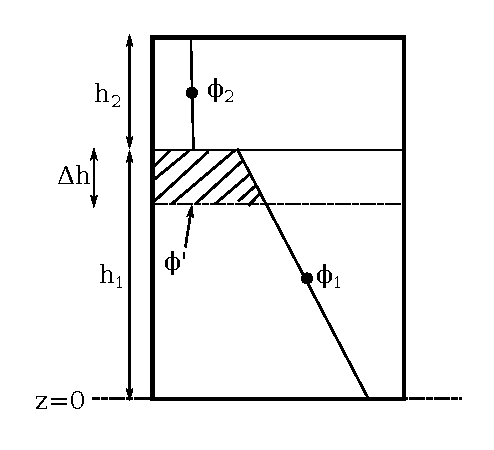
\includegraphics{../plots/schematic.pdf}
  \caption{\label{fig:schematic} A schematic demonstrating the ability for regridding/remapping to cause a decrease in RPE}
\end{figure}

\Cref{fig:schematic} shows a simple two-cell domain under regridding/remapping. The bottom cell has a mean tracer concentration of $\phi_1$ and thickness $h_1$. Similarly, the top cell has a mean tracer concentration of $\phi_2$ and thickness $h_2$. Regridding moves the interface between the cells from its initial position at $z = h_1$ to the dashed line at $z = h_1 - \Delta h$, and remapping mixes the integrated quantity of tracer $\phi'$ from the bottom cell to the top cell. Initially, the potential energy of the domain is

\begin{equation}
  PE_i = \frac{\phi_1 h_1 h_1}{2} + \phi_2 h_2\left(h_1 + \frac{h_2}{2}\right).
\end{equation}

After remapping, the potential energy becomes

\begin{equation}
  \begin{split}
    PE_f &= \left(\phi_1 h_1 - \phi'\right)\frac{h_1 - \Delta h}{2} \\
    &+ \left(\phi_2 h_2 + \phi'\right)\left(h_1 - \Delta h + \frac{h_2 + \Delta h}{2}\right).
  \end{split}
\end{equation}

Taking the difference between the final and initial potential energy gives the RPE change due to regridding/remapping,

\begin{equation}
  PE_f - PE_i = \frac{\phi'\left(h_1 + h_2\right)}{2} - \frac{\Delta h\left(\phi_1 h_1 + \phi_2 h_2\right)}{2}.
\end{equation}

With the condition that $\phi_1 > \phi_2$, it is possible for $PE_f - PE_i < 0$ when the remapping is higher order than piecewise constant (PCM). PCM is the lowest order reconstruction, and gives $\phi' = \phi_1 \Delta h$, thus $PE_f - PE_i \ge 0$.


\section{Results}
\subsection{Lock exchange}

% NOTE equivalent vertical diffusivity due to spurious mixing appears to be about 5e-6 or so
% TODO highlight that explicit vertical diffusivity is zero

The lock exchange test case (\cref{fig:lock-snapshot}) is a simple configuration that shows the creation of intermediate densities by spurious mixing. This is a replication of one of the test cases presented by \citet{ilicak12}. The test case takes place in a two-dimensional domain of 64km width and 20m depth. Only the highest resolution test cases are chosen, with horizontal and vertical grid spacings of $\Delta x = \SI{500}{\metre}$ and $\Delta z = \SI{1}{\metre}$, respectively. The lock exchange is defined by an initial temperature distribution comprised of one density class on each side of the domain,

\begin{equation}
  \Theta(x) = \begin{cases}
    \SI{5}{\celsius} & x < \SI{32}{\kilo\metre}\\
    \SI{30}{\celsius} & x \ge \SI{32}{\kilo\metre}.
  \end{cases}
\end{equation}

\begin{figure}
  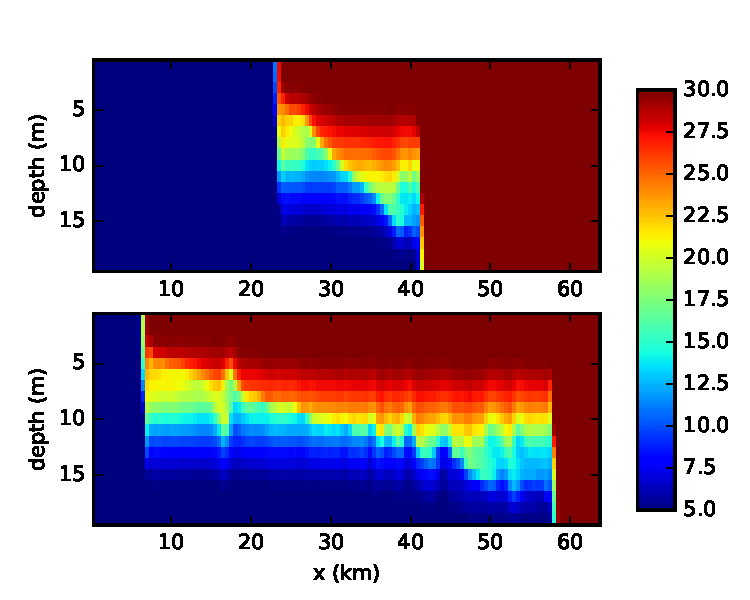
\includegraphics{{../plots/lock_exchange_snapshot_0.01}.pdf}
  \caption{\label{fig:lock-snapshot} Snapshots of lock exchange at 6 hours (top) and 17 hours (bottom) at $\nu_h = \SI{0.01}{\square\metre\per\second}$. Temperature (\si{\celsius}) is shown in colours. Spurious mixing at the front can be seen by the presence of intermediate temperatures.}
\end{figure}

This case is equivalent to two adjacent basins, each at constant temperature, with a dam between them that is removed at $t=0$. The warm water from the right basin flows from right-to-left above cold water, while conversely cold water from the left basin flows underneath the warm water from left-to-right. This is simply a gravity current, for which we have a theoretical prediction for the front velocity in a rectangular channel, given by

\begin{equation}
  u_f = \frac12 \sqrt{gH \rho'},
\end{equation}

% TODO check dimensions -- $\rho'$ should be dimensionless

where $\rho'$ is the density difference across the front. When calculating the grid Reynolds number, the theoretical front velocity is used instead of the actual mean velocity over the domain to match @ilicak12. All runs were carried out for 17 hours using a baroclinic timestep that satisfied CFL conditions across the range of horizontal viscosities (\SIlist{0.01;0.1;1;10;100;200}{\square\metre\per\second}).

\begin{figure}
  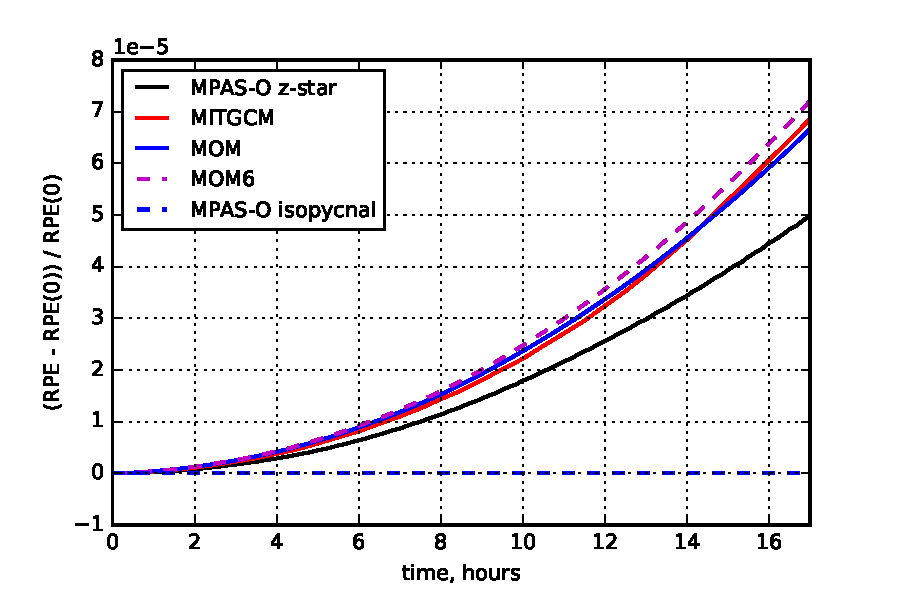
\includegraphics{../plots/lock_exchange_rpe_norm.pdf}
  \caption{\label{fig:lock-rpenorm} Normalised RPE evolution for $\nu_h = \SI{0.01}{\square\metre\per\second}$. MPAS-O, MITGCM and MOM results come from \citet{petersen15} and \citet{ilicak12}. MOM6 exhibits a larger increase in RPE due to spurious mixing.}
\end{figure}

% TODO specify which results come from which paper

\begin{figure}
  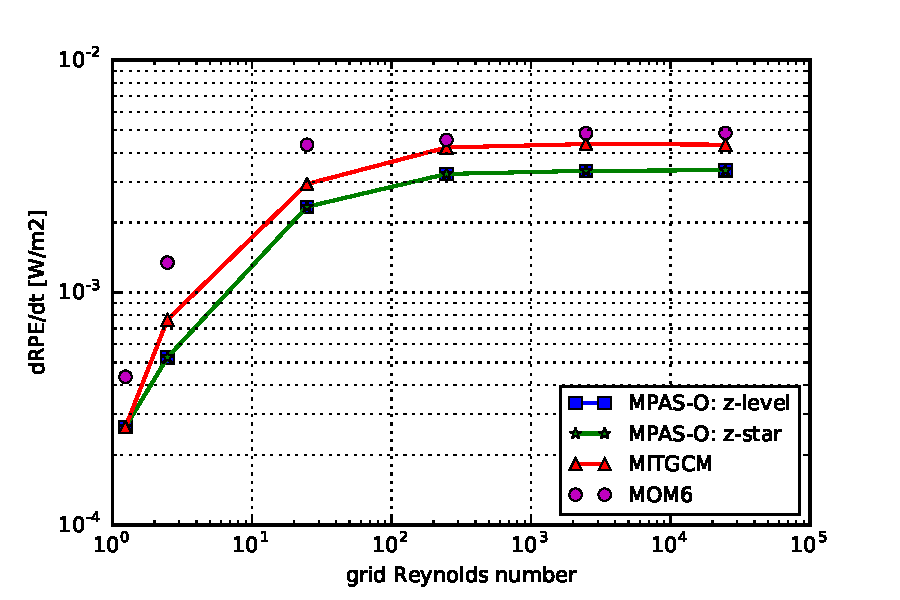
\includegraphics{../plots/lock_exchange_drpe.pdf}
  \caption{\label{fig:lock-drpe} Instantaneous rate of RPE change at 17h. MPAS-O and MITGCM results come from \citet{petersen15} and \citet{ilicak12} respectively.}
\end{figure}

% TODO place line at grid Re = 2 in this plot

The time series of normalised RPE in \cref{fig:lock-rpenorm} shows MOM6 having a similar shape to MITGCM and MOM. However, the curve steepens with time, suggesting that more spurious mixing is occurring in MOM6.

% TODO curve steepens more/values are larger in MOM6 than other models

Above a grid Reynolds number of 10, MOM6 performs somewhat worse than the other models shown in \cref{fig:lock-drpe}. At this point, the models are running above the threshold for saturation of spurious mixing. However, in the regime where spurious mixing isn't saturated, MOM6 exhibits a higher rate of RPE change. This result suggests that spurious mixing in MOM6 is due to tracer advection, as viscosity in the unsaturated regime is sufficient to damp grid-scale noise in the velocity field.

% TODO mention the cause for the "threshold for saturation of spurious mixing" -- viscosity is sufficient to damp grid-scale noise in the velocity field
% TODO look at wavenumber spectrum of velocity field

\subsubsection{Advection order}
One aspect of model configuration that may significantly affect spurious mixing is the order of accuracy of the tracer advection scheme. A higher-order advection scheme purports to reduce the spurious mixing in advection, at the cost of runtime performance. Curiously, the two advection schemes in MOM6, PLM (piecewise linear) and the Huynh third-order piecewise parabolic scheme, PPM:H3 \citep{huynh97}, exhibit nearly identical spurious mixing. In order to preserve the pre-existing range of density classes by avoiding the creation of spurious minima or maxima, advection schemes may employ limiters. In MOM6, the limiting scheme reduces to a first-order upstream method. The minimal difference in spurious mixing despite an improved advection scheme suggests that advection may be dominated by a limiter at the front, where spurious mixing is most vigorous.

% NOTE can this be checked? where is the limiter active?

\subsubsection{Directional split}
\begin{figure}
  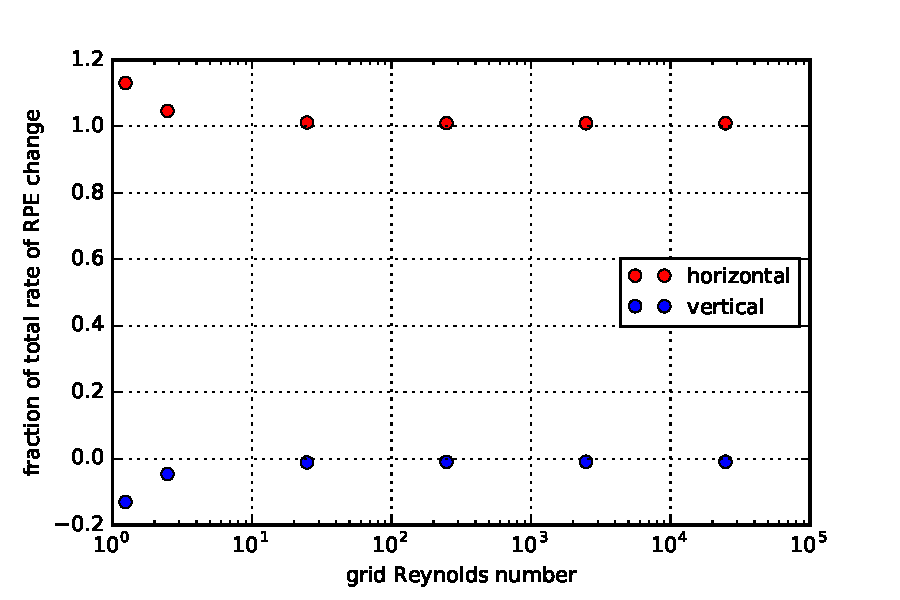
\includegraphics{../plots/lock_exchange_drpe_split.pdf}
  \caption{\label{fig:lock-rpesplit} Horizontal and vertical contributions to the instantaneous rate of RPE change at 17h}
\end{figure}

\Cref{fig:lock-rpesplit} shows that the mixing is predominantly due to horizontal processes. Indeed, for all of the experiments, the average RPE change due to regridding/remapping is actually negative. Physically, this means that regridding/remapping tends to slightly lower the centre of mass of the domain, counteracting some of the centre of mass increase due to mixing by the advection scheme. The magnitude of this compensation by regridding/remapping is negligible, so the spurious mixing is still set by the tracer advection scheme.

% TODO but MOM6 is still a little worse than other models

\subsection{Internal waves}

% TODO: mention horizontal viscosities, energy? amplitude spectrum?

The breaking of nonlinear internal waves in the ocean is a significant source of abyssal mixing, and thus is an important process contributing to the abyssal ocean circulation \citep{nikurashin13}.

- but linear waves should involve no mixing

Spurious mixing due to internal waves depends strongly on the choice of vertical coordinate. The propagation of linear internal waves produces vertical mixing in ocean models with a fixed vertical grid such as z-star \citep{gouillon10}. However, other coordinates, such as z-tilde, permit layers to move with the waves, thereby restricting transport between layers and reducing spurious mixing.

\begin{figure}
  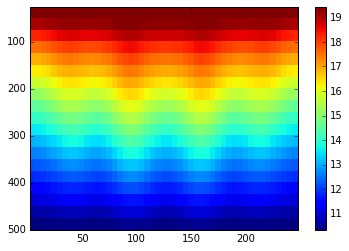
\includegraphics{{../plots/internal_waves_snapshot_0.01}.pdf}
  \caption{\label{fig:waves-snapshot} Snapshot of the internal wave initial condition (top), and state after 100 days (bottom). Temperature (\si{\celsius}) is shown in colours.}
\end{figure}

- show z-tilde and rho coords as well (4-panel)

This test case is configured as presented by \citet{ilicak12}. It consists of a linearly stratified background temperature distribution in a domain \SI{500}{\metre} deep and \SI{250}{\kilo\metre} wide (\cref{fig:waves-snapshot}). Horizontal grid spacing is \SI{5}{\kilo\metre}, and the vertical grid spacing $\Delta z$ is \SI{25}{\metre}. A wave perturbation is superimposed, lifting the isopycnals in the centre of the domain to set up counter-propagating internal waves towards the left and right horizontal boundaries. The background temperature distribution is defined as

\begin{equation}
  \Theta_0(z) = \Theta_\text{bot} + (\Theta_\text{top} - \Theta_\text{bot})\frac{z_\text{bot} - z}{z_\text{bot}},
\end{equation}

where $\Theta_\text{bot} = 10.1^\circ\mathrm{C}$, $\Theta_\text{top} = \SI{20.1}{\celsius}$, and $z_\text{bot} = \SI{-487.5}{\metre}$. The wave perturbation,

- mention coordinate convention on z (z coordinate relative to surface)
- explain discrepancy in $z_\text{bot}$ due to staggered grid

\begin{equation}
  \Theta'(x,z) = -A\cos\left(\frac{\pi}{2L}(x - x_0)\right) \sin\left(\pi\frac{z + \Delta z/2}{z_\text{bot} + \Delta z/2}\right),
\end{equation}

is added in the region $x_0 - L < x < x_0 + L$, where $L = \SI{50}{\kilo\metre}$, $x_0 = \SI{125}{\kilo\metre}$. Only the high-amplitude case, with perturbation amplitude $A = \SI{2}{\celsius}$ is used, as it is the only case also presented by \citet{petersen15}. The waves set up by this perturbation have a period of approximately one day, so the test case is run for 100 days to allow the waves to propagate many times across the full extent of the domain.

- mention buoyancy frequency, or remove "propagation time"

\begin{figure}
  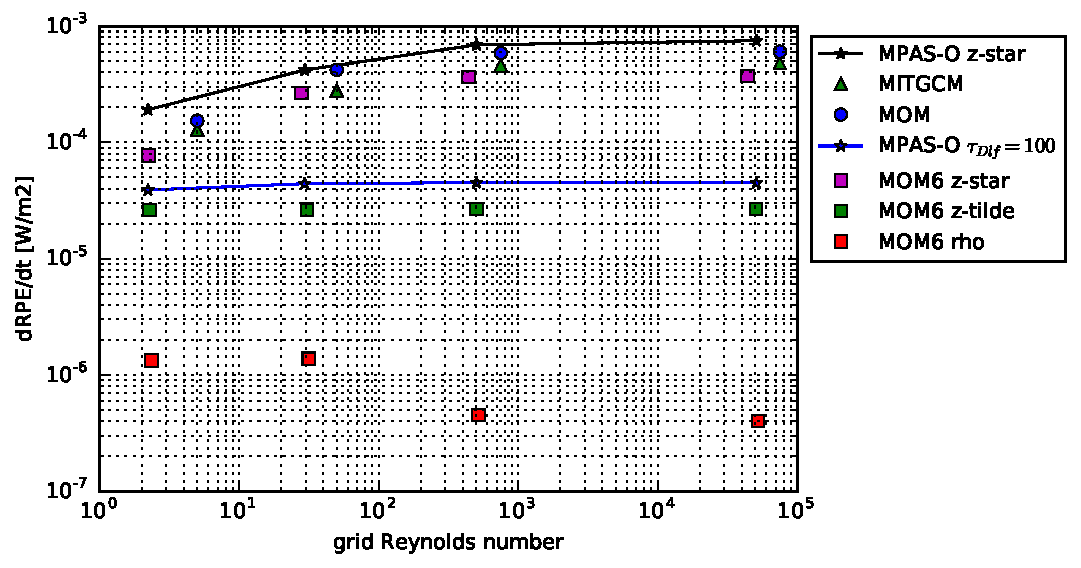
\includegraphics{../plots/internal_waves_drpe.pdf}
  \caption{\label{fig:waves-drpe} Averaged rate of RPE change from 10 to 100 days in internal waves test case. MPAS-O, MITGCM and MOM results come from \citet{petersen15} and \citet{ilicak12}. MOM6 is shown with square markers, in magenta for z-star, green for z-tilde and red for continuous isopycnal. MOM6 performs comparably or better to models using the same vertical coordinate, and shows a significant reduction in spurious mixing with the continuous isopycnal coordinate.}
\end{figure}

- state which results come from which model
- specify default MOM6 case is z-star

Considering the average rate of RPE change (\cref{fig:waves-drpe}), MOM6 performs well for each of the chosen vertical coordinates; z-star, z-tilde and continuous isopycnal (rho). This is likely due to its implementation as a quasi-Lagrangian ALE model. In this configuration, vertical layers are able to move freely within their column as waves pass through. During horizontal advection, there is exactly zero transport through vertical interfaces, so mixing occurs only laterally along an isopycnal layer. The vertical coordinate becomes more isopycnal with the z-tilde and rho coordinates, thus regridding causes smaller displacement of the interfaces. Subsequently, there is less vertical transport due to remapping and the overall spurious mixing is reduced.

The implementation of the z-tilde coordinate differs between MOM6 and MPAS-O. The filter timescale $\tau_{Dlf}$ in MPAS-O defines the cutoff above which frequencies are treated in a Lagrangian manner. As MOM6 is a layered model, all motion is Lagrangian during a single timestep. The only controllable parameter in the MOM6 implementation of z-tilde is $\tau_{hhf}$, which defines the relaxation timescale of the grid, to prevent long-term drift. We set this to 30 days to match the configuration used for MPAS-O. MOM6 exhibits only a modest improvement over MPAS-O here, since most dynamically interesting scales are already captured by the 100 day Lagrangian timescale $\tau_{Dlf}$ used by MPAS-O.

\subsubsection{Spurious mixing orientation}

\begin{figure}
  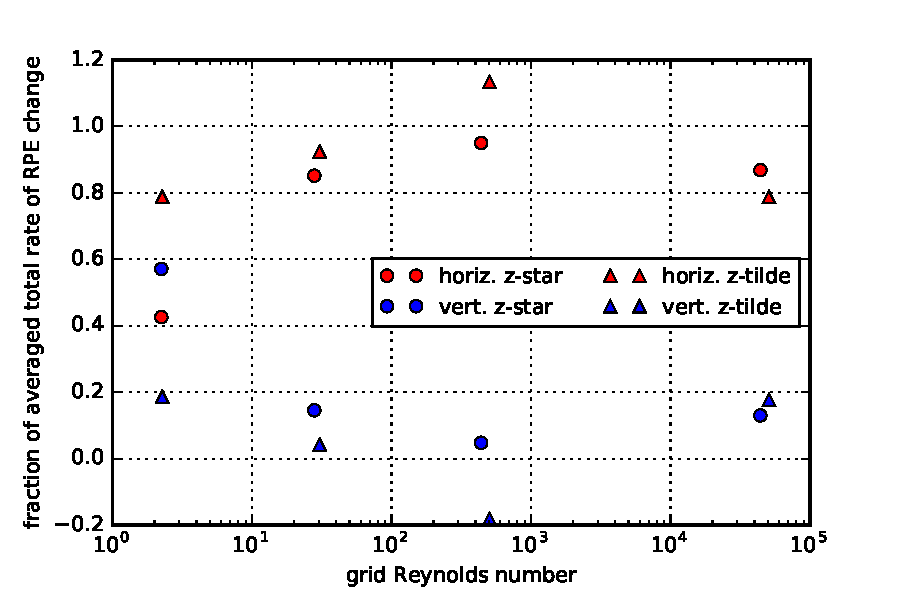
\includegraphics{../plots/internal_waves_drpe_split.pdf}
  \caption{\label{fig:waves-drpesplit} Relative contributions to spurious mixing by horizontal and vertical processes in internal waves test case. Each contribution is the fraction of the time-averaged total rate of RPE change.}
\end{figure}

- star symbol for z-star
- caption details

We take the z-star configuration of MOM6 (shown in magenta in \cref{fig:waves-drpe}) and compute the orientation of the spurious mixing, shown in \cref{fig:waves-drpesplit}. When $\mathrm{Re}_\Delta < 10$, the horizontal component is smaller than the vertical. This is consistent with the conclusion of \citet{ilicak12}, that the grid Reynolds number must be below 10 to avoid the saturation level of spurious mixing. In this regime, the vertical configuration such as coordinate or reconstruction accuracy can have a significant impact on the overall spurious mixing. There is a minimum in the vertical contribution at $\nu_h = \SI{1}{\square\metre\per\second}$, corresponding to $\mathrm{Re}_\Delta \approx 400$.

- why?

\Cref{fig:waves-drpesplit} shows the relative contributions to the total rate of RPE change by the horizontal and vertical components. There is once again a minimum in the contribution by the vertical component at $\nu_h = \SI{1}{\square\metre\per\second}$, corresponding to $\mathrm{Re}_\Delta \approx 400$. Since this also happens with the z-star and continuous isopycnal coordinates (\cref{fig:waves-drpe}), it is mostly likely a feedback effect or resonance due to the horizontal viscosity.

\subsection{Baroclinic eddies}

% TODO: mention \Delta z

The previous two test cases were only two-dimensional, and therefore couldn't incorporate the influence of the Coriolis force. We now introduce a test case that involves a baroclinically unstable temperature front in a periodic channel with rotation. This test case was presented by \citet{ilicak12}, as the baroclinically unstable front quickly leads to vigorous eddying without either mechanical or buoyancy forcing, thus it is a closed system suitable for analysis by changes in RPE. The domain is a periodic channel in the x direction, \SI{160}{\kilo\metre} wide by \SI{500}{\kilo\metre} long, with a depth of \SI{1000}{\metre} (\cref{fig:eddies-snapshot_ic}). The front has a sinusoidal initial meridional position, defined as

\begin{equation}
  y_w(x) = y_0 - y_A \sin\left(2\pi k \frac{x}{L_x}\right),
\end{equation}

where $y_A = \SI{40}{\kilo\metre}$ is the amplitude, $y_0 = \SI{250}{\kilo\metre}$ is the centre of the domain, $k = 3$ and $L_x = \SI{160}{\kilo\metre}$ ensure that three wavelengths span the width of the domain. The initial temperature distribution in the domain is given by

\begin{equation}
  \Theta(x,y,z) = \begin{cases}
    \Theta_0(z) & y \ge y_w(x) + \Delta y, \\
    \Theta_0(z) - \Delta \Theta \left(1 - \frac{y - y_w(x)}{\Delta y}\right) & y_w < y < y_w + \Delta y, \\
    \Theta_0(z) - \Delta \Theta & y \le y_w(x),
  \end{cases}
\end{equation}

where $\Theta_0(z)$ is a linearly stratified background between \SI{10.1}{\celsius} and \SI{13.1}{\celsius}, $\Delta y = \SI{40}{\kilo\metre}$ is the width of the front and $\Delta \Theta = \SI{1.2}{\celsius}$ is the temperature difference across the front. Additionally, a temperature perturbation is added to the crest of one of the waves to promote instability. The region over which the perturbation is added is bounded by $x_2 \le x \le x_3$ and $y'_w - \Delta y / 2 \le y \le y'_w + \Delta y / 2$, where

\begin{equation}
  y'_w(x) = y_0 - \frac{y_A}{2}\sin\left(\pi \frac{x - x_2}{x_3 - x_2}\right).
\end{equation}

\begin{figure}
  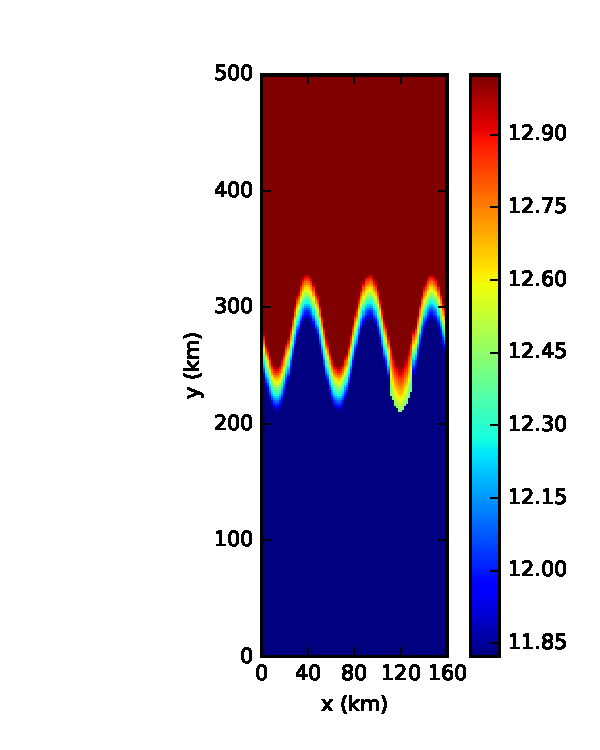
\includegraphics{../plots/eddies_snapshot_dx1_initial.pdf}
  \caption{\label{fig:eddies-snapshot_ic} Snapshot of initial condition of surface temperature for the baroclinic eddies test case at \SI{1}{\kilo\metre} horizontal resolution. The temperature perturbation can be seen at the third trough in the sinusoidal front.}
\end{figure}

\begin{figure}
  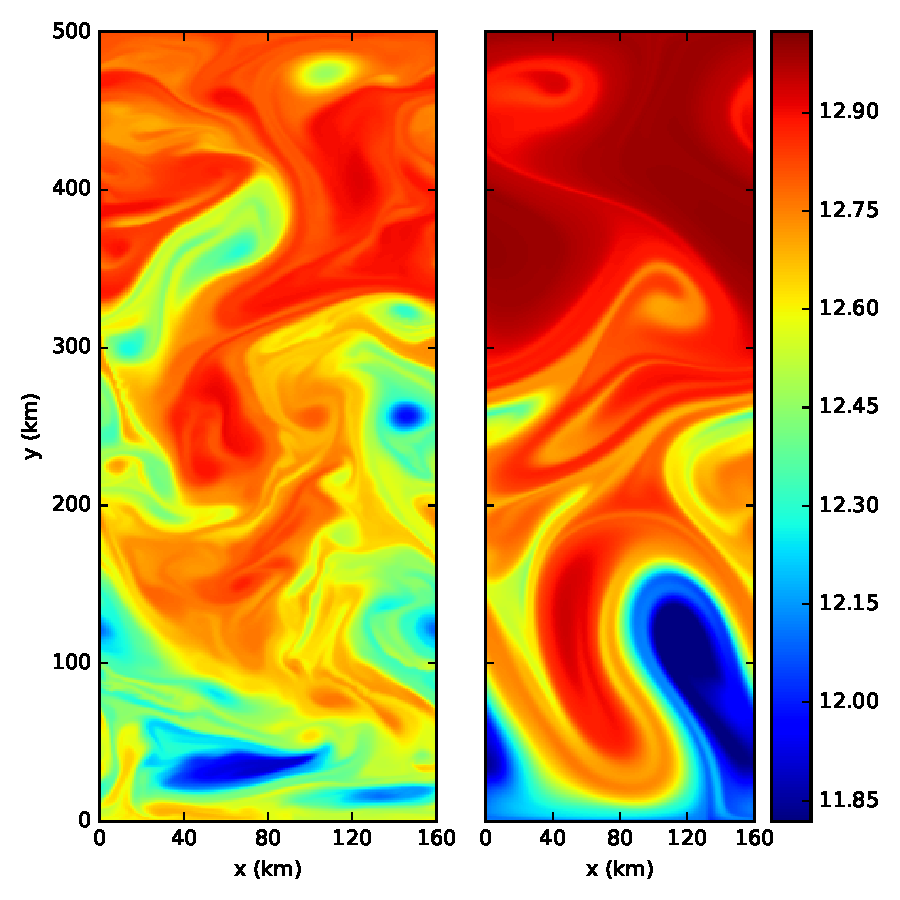
\includegraphics{../plots/eddies_snapshot_dx1.pdf}
  \caption{\label{fig:eddies-snapshot} Snapshots of surface temperature (\si{\celsius}) after 320 days of simulation at \SI{1}{\kilo\metre} horizontal resolution. Left panel is low viscosity (high grid Reynolds number), $\nu_h = \SI{1}{\square\metre\per\second}$. Right panel is high viscosity (low grid Reynolds number), $\nu_h = \SI{200}{\square\metre\per\second}$. There is more mixing at low viscosities, but the features are finer in scale.}
\end{figure}

The perturbation itself is defined by the temperature anomaly

\begin{equation}
  \Theta'(x,y) = \Delta\Theta'\left(1 - \frac{y - y'_w(x)}{\Delta y / 2}\right).
\end{equation}

In order to encourage baroclinicity, a quadratic bottom drag with drag coefficient $C_D = 0.01$ is used. Experiments were performed at horizontal resolutions of \SIlist{1;4;10}{\kilo\metre}. For each choice of horizontal resolution, the horizontal viscosities $\nu_h$ were \SIlist{1;5;10;20;200}{\square\metre\per\second}, giving a range of lateral grid Reynolds numbers from $O(1)$ at the highest viscosity, through to $O(1000)$ for the lowest viscosity.

\Cref{fig:eddies-snapshot} shows the surface temperature after the full 320 days of simulation at 1km horizontal resolution, at the lowest and highest viscosities, \SI{1}{\square\metre\per\second} and \SI{200}{\square\metre\per\second}, respectively. In the low viscosity case, strong spurious mixing has occurred, but finer-scale features are also evident. Conversely, the range of intermediate temperatures is significantly less with a higher horizontal viscosity, but the eddies are much weaker due to the momentum damping by the viscosity.

\begin{figure}
  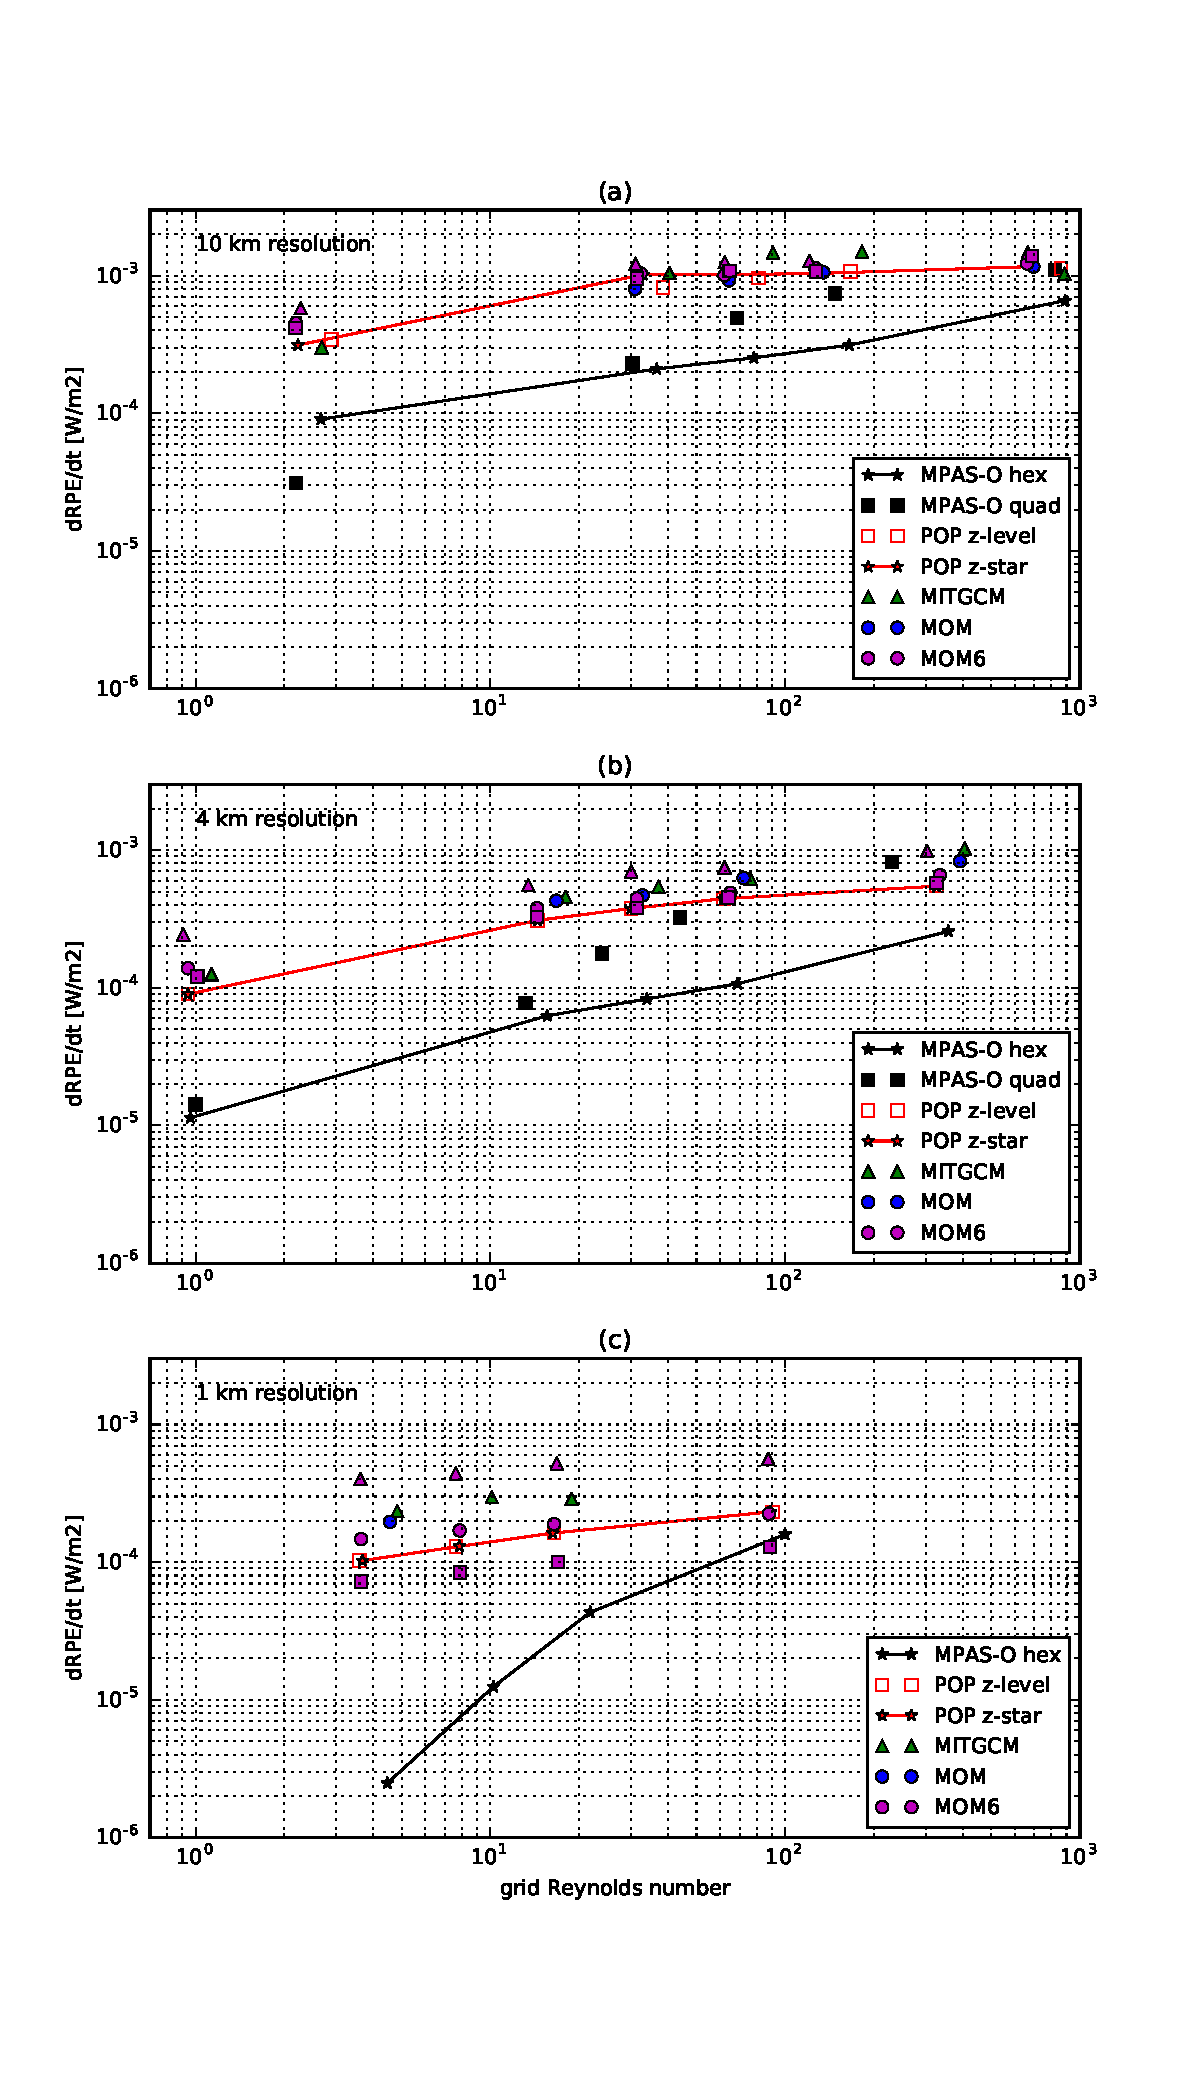
\includegraphics{../plots/eddies_drpe.pdf}
  \caption{\label{fig:eddies-drpe} Rate of RPE change for all experiments. Data from MPAS-O, POP, MITGCM and MOM come from @petersen15 and @ilicak12. MOM6 using the default PLM tracer advection scheme is shown in magenta circles, with the alternate PPM:H3 scheme shown in magenta triangles at \SIlist{10;4}{\kilo\metre} resolution.}
\end{figure}

\Cref{fig:eddies-drpe} shows the rate of RPE change across all tested models for \SIlist{10;4;1}{\kilo\metre} horizontal resolution, respectively. In the 10km experiment, the two available tracer advection schemes were used, PLM shown in magenta circles and the higher-order PPM:H3 scheme in magenta triangles. In the spurious mixing saturation regime of $\mathrm{Re}_\Delta > 10$, MOM6 with the PLM scheme plateaus at a very similar level to MOM and POP. As expected, the PPM:H3 scheme exhibits slightly lower spurious mixing, especially at the lowest grid Reynolds number. However, in the saturation regime the spurious mixing continues to rise slightly with increasing grid Reynolds number, exceeding the PLM scheme.

When the horizontal resolution is decreased to 4km, MOM6 exhibits slightly greater spurious mixing than POP across the range of experiments. At this resolution, the PPM:H3 advection scheme consistently provides a small decrease in spurious mixing as compared to the PLM scheme. However, the improvement in spurious mixing is minor, and may not be worth the extra computational cost involved in invoking the PPM:H3 advection scheme.

\subsubsection{Spurious mixing orientation}

\begin{figure}
  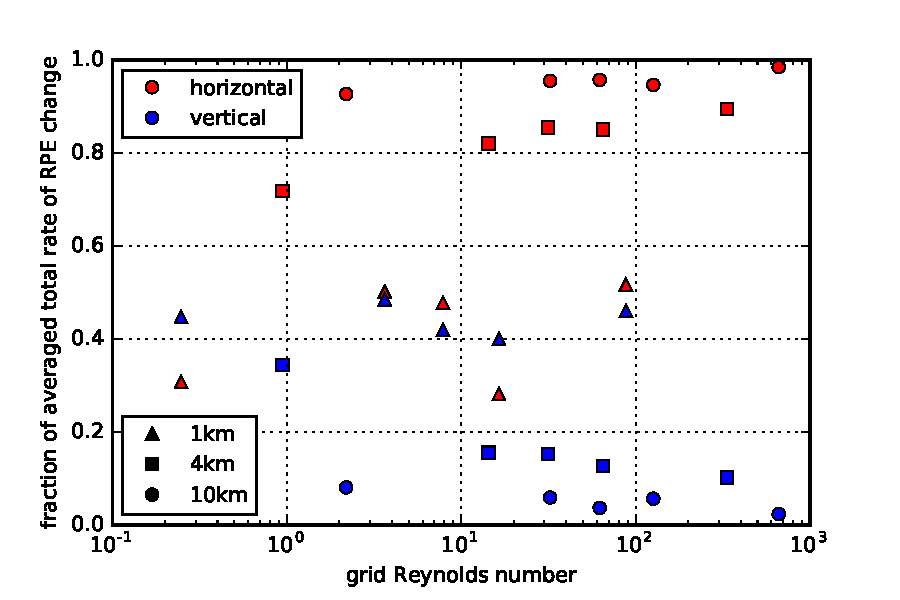
\includegraphics{../plots/eddies_drpe_split.pdf}
  \caption{\label{fig:eddies-drpesplit} Spurious mixing contributions in MOM6 for each horizontal resolution across the range of horizontal viscosities. \SI{1}{\kilo\metre} shown with triangles, \SI{4}{\kilo\metre} with squares and \SI{10}{\kilo\metre} with circles. As resolution increases, the relative contribution of the vertical component also increases, to approximately equal the horizontal component at \SI{1}{\kilo\metre}.}
\end{figure}

- make sure legend is fixed

We consider the orientation of spurious mixing at each of the tested horizontal resolutions in \cref{fig:eddies-drpesplit}. As horizontal resolution increases (grid spacing decreases), the fraction of spurious mixing by regridding/remapping increases. Indeed, at \SI{1}{\kilo\metre} horizontal resolution, horizontal tracer advection and regridding/remapping contribute approximately equally to the total spurious mixing. The reasons for this are likely twofold: firstly, for the same domain size at higher resolution, there are simply more water columns in which regridding/remapping must take place. Secondly, fine-scale features in the flow may cause more interaction between adjacent water columns, or more rapid changes in the Lagrangian vertical grid which require correction by regridding/remapping. This result highlights the importance of further refinement of regridding/remapping schemes and vertical coordinates, particularly as models are run at increasingly higher resolution.

- "anti-spurious mixing"


\section{Discussion}
% TODO expand points

\subsection{Horizontal resolution}
With increasing horizontal resolution, the fraction of spurious mixing contributed by vertical processes increases. As shown in \cref{fig:eddies-drpe}, a fourfold reduction in horizontal resolution only leads to a halving of the total magnitude of the spurious mixing rate.

\subsection{Vertical resolution}
The magnitude of spurious mixing scales approximately linearly with vertical resolution. In combination with the conclusion mentioned above, the 

\subsection{Advection scheme}
The two tracer advection schemes in MOM6, PLM and PPM:H3, don't appear to be sufficient for traditional coordinate systems. Here, tracers may vary significantly in a single layer, and the advantages of being able to solve the primitive equations in generalised vertical coordinates are lost.

\subsection{Coordinate choice}
By far the most important contribution to the magnitude of spurious mixing tested here is the choice of vertical coordinate. Generalised coordinates such as z-tilde or continuous isopycnal showed significant improvements over the ubiquitous z-star coordinate used in ocean models. However, these are not instant solutions; they require tuning to perform optimally, and additionally have more stringent stability and configuration requirements.

\section{Conclusions}


\section*{References}

\bibliography{bibliography}

\end{document}
